% ============================================================================
% AOGS model schematic — the poster's anchor visual: the two advances in one
% physical picture. Left: terrain horizon blocks the low sun (ray-traced from
% the LOLA DEM). Right: the 3-layer regolith column, surface energy balance,
% HFE borestem sensors, and the basal flux anchor.
% Depth NOT to scale (layers exaggerated so z1/z2 are visible).
% Numbers: sweep ranges + Q_b from code/src/lunar/config.py; K(T,z) form
% Hayne et al. 2017. House palette (lunar.plotting.style).
% Build:  /Library/TeX/texbin/pdflatex aogs_model_schematic.tex
% PNG:    python3 -c "import fitz; fitz.open('aogs_model_schematic.pdf')[0].get_pixmap(dpi=300).save('aogs_model_schematic.png')"
% ============================================================================
\documentclass[tikz, border=8pt]{standalone}
\usepackage[T1]{fontenc}
\usepackage{newtxtext,newtxmath}
\usetikzlibrary{positioning, arrows.meta, calc, decorations.pathreplacing}

% house palette (lunar.plotting.style)
\definecolor{teal}{HTML}{2A6478}
\definecolor{coral}{HTML}{B85B3A}
\definecolor{forest}{HTML}{3D6E4A}
\definecolor{char}{HTML}{2A2520}
\definecolor{gridc}{HTML}{E8E5E0}
\definecolor{dim}{HTML}{8A857E}
\definecolor{cream}{HTML}{F7F5F1}

\begin{document}
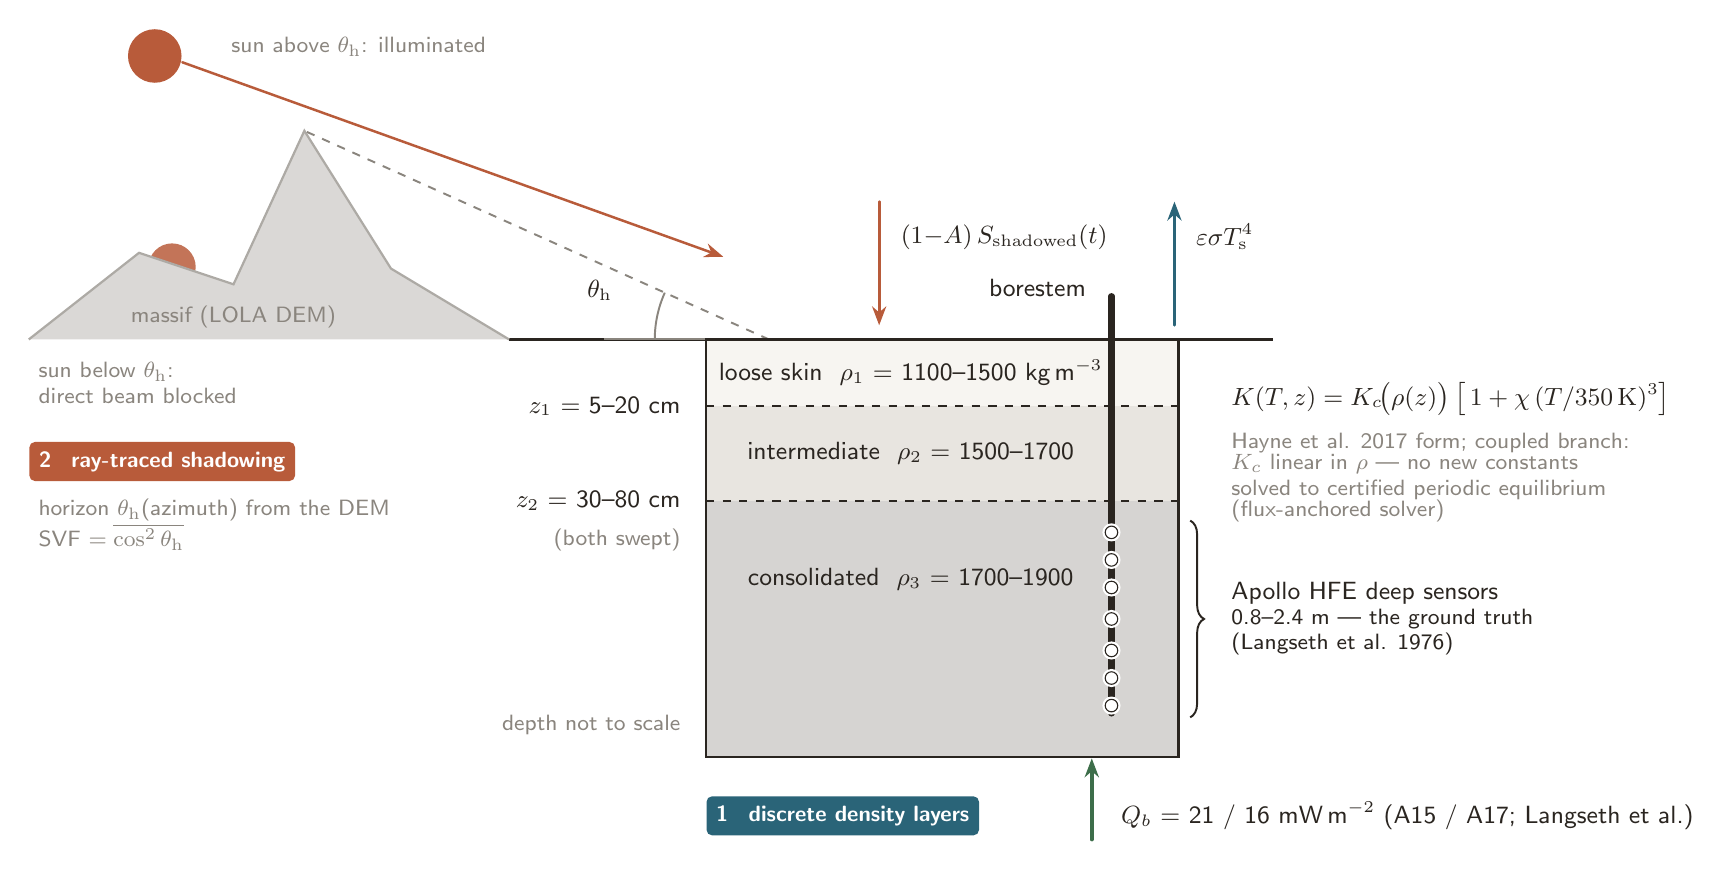
\begin{tikzpicture}[
  font=\sffamily,
  lbl/.style={font=\sffamily\small, text=char},
  sub/.style={font=\sffamily\footnotesize, text=dim},
  chip/.style={fill=#1, text=white, font=\sffamily\bfseries\small,
               rounded corners=2pt, inner sep=3.5pt},
  arr/.style={-{Stealth[length=2.4mm]}, line width=1.0pt, line cap=round},
]

% ─── surface line ────────────────────────────────────────────────────────────
\draw[char, line width=1.2pt] (4.9, 0) -- (14.6, 0);

% ─── terrain (left): massif + horizon ───────────────────────────────────────
% blocked sun FIRST, so the massif fill covers its lower half (a low sun
% still hidden behind the ridge — the blocked geometry, with no stub ray)
\fill[coral!85] (0.62, 0.92) circle (0.30);
\fill[dim!32] (-1.2, 0) -- (0.2, 1.1) -- (1.4, 0.7) -- (2.3, 2.65)
              -- (3.4, 0.9) -- (4.9, 0) -- (-1.2, 0) -- cycle;
\draw[dim!70, line width=0.8pt] (-1.2, 0) -- (0.2, 1.1) -- (1.4, 0.7)
              -- (2.3, 2.65) -- (3.4, 0.9) -- (4.9, 0);
\node[sub] at (1.4, 0.28) {massif (LOLA DEM)};

% horizon ray from the surface point to the peak + angle
\coordinate (P) at (8.2, 0);
\draw[dim, dashed, line width=0.7pt] (P) -- (2.3, 2.65);
\draw[dim, line width=0.7pt] (P) -- ++(-2.1, 0);
\draw[dim, line width=0.7pt] ($(P)+(-1.45,0)$) arc[start angle=180,
      end angle=155.8, radius=1.45];
\node[lbl] at (6.05, 0.62) {$\theta_{\mathrm{h}}$};

\node[sub, align=left, anchor=west] at (-1.2, -0.55)
      {sun below $\theta_{\mathrm{h}}$:\\ direct beam blocked};

% clear sun: above the horizon ray
\fill[coral] (0.4, 3.6) circle (0.34);
\draw[coral, arr, line width=0.9pt] (0.75, 3.52) -- (7.62, 1.05);
\node[sub, anchor=west] at (1.25, 3.72) {sun above $\theta_{\mathrm{h}}$: illuminated};

% chip + SVF note live BELOW ground level on the empty left — nothing to
% strike through them there
\node[chip=coral, anchor=west] at (-1.2, -1.55)
      {\footnotesize 2 \, ray-traced shadowing};
\node[sub, anchor=west, align=left] at (-1.2, -2.35)
      {horizon $\theta_{\mathrm{h}}$(azimuth) from the DEM\\
       SVF $=\overline{\cos^2\theta_{\mathrm{h}}}$};

% ─── surface energy balance ─────────────────────────────────────────────────
\draw[coral, arr] (9.6, 1.75) -- (9.6, 0.18);
\node[lbl, anchor=west] at (9.75, 1.30) {$(1{-}A)\,S_{\mathrm{shadowed}}(t)$};
\draw[teal, arr] (13.35, 0.18) -- (13.35, 1.75);
\node[lbl, anchor=west] at (13.5, 1.30) {$\varepsilon\sigma T_{\mathrm{s}}^{4}$};

% ─── regolith column (depth exaggerated) ────────────────────────────────────
\fill[cream]    (7.4, -0.85) rectangle (13.4, 0);
\fill[gridc]    (7.4, -2.05) rectangle (13.4, -0.85);
\fill[dim!35]   (7.4, -5.30) rectangle (13.4, -2.05);
\draw[char, line width=0.9pt] (7.4, -5.30) rectangle (13.4, 0);
\draw[char, dashed, line width=0.7pt] (7.4, -0.85) -- (13.4, -0.85);
\draw[char, dashed, line width=0.7pt] (7.4, -2.05) -- (13.4, -2.05);

\node[lbl] at (10.0, -0.42)
      {loose skin \ $\rho_1$ = 1100--1500 kg\,m$^{-3}$};
\node[lbl] at (10.0, -1.45)
      {intermediate \ $\rho_2$ = 1500--1700};
\node[lbl] at (10.0, -3.05)
      {consolidated \ $\rho_3$ = 1700--1900};

% boundary labels (left of column)
\node[lbl, anchor=east] at (7.2, -0.85) {$z_1$ = 5--20 cm};
\node[lbl, anchor=east] at (7.2, -2.05) {$z_2$ = 30--80 cm};
\node[sub, anchor=east] at (7.2, -2.55) {(both swept)};
\node[sub, anchor=east] at (7.2, -4.9) {depth not to scale};

\node[chip=teal, anchor=west] at (7.4, -6.05)
      {\footnotesize 1 \, discrete density layers};

% ─── HFE borestem + sensors ─────────────────────────────────────────────────
\draw[char, line width=2.2pt, line cap=round] (12.55, 0.55) -- (12.55, -4.75);
\foreach \y in {-2.45, -2.80, -3.15, -3.55, -3.95, -4.30, -4.65}
  \fill[white] (12.55, \y) circle (0.115)
  (12.55, \y) circle (0.115) node[draw=char, circle, inner sep=1.6pt] {};
\draw[decorate, decoration={brace, amplitude=5pt}, char, line width=0.7pt]
      (13.55, -2.30) -- (13.55, -4.80);
\node[lbl, anchor=west, align=left] at (13.95, -3.55)
      {Apollo HFE deep sensors\\[-2pt]
       {\footnotesize 0.8--2.4 m — the ground truth}\\[-2pt]
       {\footnotesize (Langseth et al. 1976)}};
\node[lbl, anchor=south east] at (12.35, 0.42) {borestem};

% ─── conductivity law (right of column) ─────────────────────────────────────
\node[lbl, anchor=west, align=left] at (13.95, -0.75)
      {$K(T,z) = K_c\!\big(\rho(z)\big)\,
        \big[\,1 + \chi\,(T/350\,\mathrm{K})^{3}\big]$};
\node[sub, anchor=west, align=left] at (13.95, -1.45)
      {Hayne et al. 2017 form; coupled branch:\\[-2pt]
       $K_c$ linear in $\rho$ — no new constants};
\node[sub, anchor=west, align=left] at (13.95, -2.05)
      {solved to certified periodic equilibrium\\[-2pt]
       (flux-anchored solver)};

% ─── basal flux ──────────────────────────────────────────────────────────────
\draw[forest, arr, line width=1.4pt] (12.3, -6.35) -- (12.3, -5.32);
\node[lbl, anchor=west] at (12.55, -6.05)
      {$Q_b$ = 21 / 16 mW\,m$^{-2}$ (A15 / A17; Langseth et al.)};

\end{tikzpicture}
\end{document}
